% !!! 如果要编译此文件,请确定已经安装了 elegantnote。 对于 texlive 用户,可以使用
% tlmgr install elegantnote
% 进行安装
\documentclass[blue,normal,cn]{elegantnote}
%\usepackage{lstlisting}
\usepackage{pdfpages}
\newfontfamily\courier{Courier New}
\lstset{linewidth=1.1\textwidth,
	numbers=left,
	basicstyle=\small\courier,
	numberstyle=\tiny\courier,
	keywordstyle=\color{blue}\courier,
	commentstyle=\it\color[cmyk]{1,0,1,0}\courier, 
	stringstyle=\it\color[RGB]{128,0,0}\courier,
	frame=single,
	backgroundcolor=\color[RGB]{245,245,244},
	breaklines,
	extendedchars=false, 
	xleftmargin=2em,xrightmargin=2em, aboveskip=1em,
	tabsize=4, 
	showspaces=false
	basicstyle=\small\courier
}
\title{语法分析程序的设计与实现}
\version{$\epsilon$}
\date{\today}
\author{2017211305班\ 2017211240\ 于海鑫}

\begin{document}
\maketitle
本文档为编译原理课程实验``语法分析程序的设计与实现''的实验报告。

\section{实验题目}
\subsection{题目}
语法程序的设计与实现
\subsection{实验内容}
编写语法分析程序,实现对算数表达式的语法解析。我们要分析的文法
如下:
$$
E \to E + T \ |\  E - T\ |\  T
$$
$$
T \to T * F \ |\  T / F\ |\  F
$$
$$
F \to (E) \ |\  id
$$
\subsection{实验要求}
在对输入表达式进行分析的过程中,输出所采用的生成式。使用如下方法:
\begin{itemize}
	\item 编写 $LL(1)$ 语法分析程序,要求如下:
	\begin{enumerate}
		\item 编程实现算法 \textbf{4.2},为给定文法自动构造预测分析表
		\item 编程实现算法 \textbf{4.1},构造 $LL(1)$ 预测分析程序
	\end{enumerate}
	\item 编写语法分析程序实现自底向上的分析,要求如下:
	\begin{enumerate}
		\item 构造识别所有或前缀的 DFA
		\item 构造 LR 分析表
		\item 编程实现算法 \textbf{4.3},构造 LR 分析程序
	\end{enumerate}
\end{itemize}

\section{实验分析}
本次实验我们实现了如上所述两种方法。其中使用的词法分析使用了词法分析
类,我们使用的词法分析类如下:

\begin{lstlisting}[language=python]
class Lexer:
    def __init__(self, expression):
        self.token = None
        self.expression = (expression + '$').replace(" ", "")

    def next_token(self):
        if self.token:
            temp = self.token
            self.token = None
            return temp
        else:
            return self._next_token()

    def peek_token(self):
        if not self.token:
            self.token = self._next_token()
        return self.token

    def _next_token(self):
        if self.expression == '':
            return None
        c = self.expression[0]
        if c == '(' or c == ')' or c == '+' or c == '-' or c == '*' or c == '/' or c == '$':
            self.expression = self.expression[1:]
            return c
        else:
            result = None
            i = 1
            try:
                while i < len(self.expression):
                    if self.expression[i - 1] == '.':
                        i += 1
                    result = float(self.expression[:i])
                    i += 1
            except:
                self.expression = self.expression[i - 1:]
                return 'n'#result
        t = len(self.expression)
        self.expression = self.expression[i - 1:]
        return 'n' if i == t else result
\end{lstlisting}

\section{$LL(1)$ 语法分析}

\subsection{实验原理}
构造分析表的方法如图~\ref{fig:4.2}~所示。

\begin{figure}[!htbp]
    \centering
    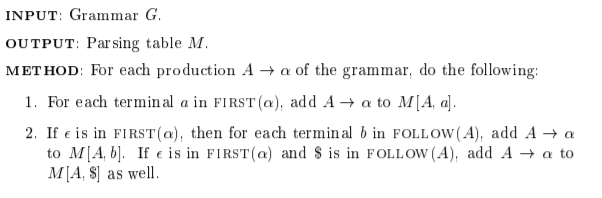
\includegraphics[width=.8\textwidth]{A.png}
    \caption{构造分析表}
    \label{fig:4.2}
\end{figure}

在构造分析表之前,我们还需要进行几个步骤:
\begin{enumerate}
	\item 消除左递归
	\item 构造 $FIRST$ 集,$FOLLOW$ 集
\end{enumerate}

所谓消除左递归,就是类似将 $E \to E + T\ |\ T$ 转化为 $E \to TE'$ 以及
$E' \to + TE'\ |\ \epsilon$ 的操作,这部分很容易使用编程语言实现。

计算 $FIRST$ 集以及 $FOLLOW$ 集则按照定义计算即可。

在获取了预测表之后,我们就可以使用如算法\textbf{4.1} 所述的
方式进行语法解析。

\subsection{数据结构}
为了实现预测分析程序,我们需要设计一套数据结构用以保存语法、预测分析表以及
转换的状态。

\subsubsection{语法}

对于语法,我们需要保存其生成式以及起始符号等信息,其定义如下:

\begin{lstlisting}[language=python]
class Grammer:
    def __init__(self):
        self.startSymbol = 'S' # default start symbol
        self.nonTerminalSymbol = set()
        self.terminalSymbol = set()
        self.generatorExpression = {}

        # Temp variable
        self.nullable = {}
        self.firstSymbols = {}
        self.followSymbols = {}
        self.llTable = {}
\end{lstlisting}


\subsubsection{预测分析表}
预测分析表实际上是一个二维字典,不再详细介绍。

\subsubsection{转换程序}
在转换程序内,我们要保存之前生成的预测分析表以及分析时所需的栈,定义如下:

\begin{lstlisting}[language=python]
class LLParser:
    def __init__(self, grammer,expression):
        self.grammer = grammer
        self.lexer = Lexer(expression)
        self.stack = ['$', self.grammer.startSymbol]
\end{lstlisting}

其中的 \texttt{lexer} 是我们的词法分析器。

\subsection{算法实现}

实现与书上一致。主要代码如下:
\lstinputlisting[language=python]{LL1/Grammer.py}

\subsection{运行结果}

我们以解析 \texttt{(1 + 2) + 2.5} 为例,程序的输出如下:

\begin{lstlisting}
PS D:\playground\FCalculator> python .\LL1\Grammer.py
{'E': ['E+T', 'E-T', 'T'], 'T': ['T*F', 'T/F', 'F'], 'F': ['(E)', 'n']}
{'E': ['TA'], 'T': ['FB'], 'F': ['(E)', 'n'], 'A': ['+TA', '-TA', ''], 'B': ['*FB', '/FB', '']}
{'E': False, 'F': False, 'B': True, 'T': False, 'A': True}
{'E': {'n', '('}, 'F': {'n', '('}, 'B': {'', '/', '*'}, 'T': {'n', '('}, 'A': {'', '+', '-'}}
{'E': {')', '$'}, 'F': {'/', '*', ')', '-', '+', '$'}, 'B': {')', '-', '+', '$'}, 'T': {')', '-', '+', '$'}, 'A': {')', '$'}}
{'E': {'n': 'TA', '(': 'TA'}, 'F': {'(': '(E)', 'n': 'n'}, 'B': {'*': '*FB', '/': '/FB', ')': '', '-': '', '+': '', '$': ''}, 'T': {'n': 'FB', '(': 'FB'}, 'A': {'+': '+TA', '-': '-TA', ')': '', '$': ''}}
E -> TA
T -> FB
F -> (E)
E -> TA
T -> FB
F -> n
B -> ''
A -> +TA
T -> FB
F -> n
B -> ''
A -> ''
B -> ''
A -> +TA
T -> FB
F -> n
B -> ''
A -> ''
\end{lstlisting}

其中 '' 表示 $\epsilon$,输出与预测一致。

\section{$LR$ 语法分析}

\subsection{实验原理}
我们首先构造识别文法的 DFA,如图~\ref{fig:5}~。

\begin{figure}[!htbp]
    \centering
    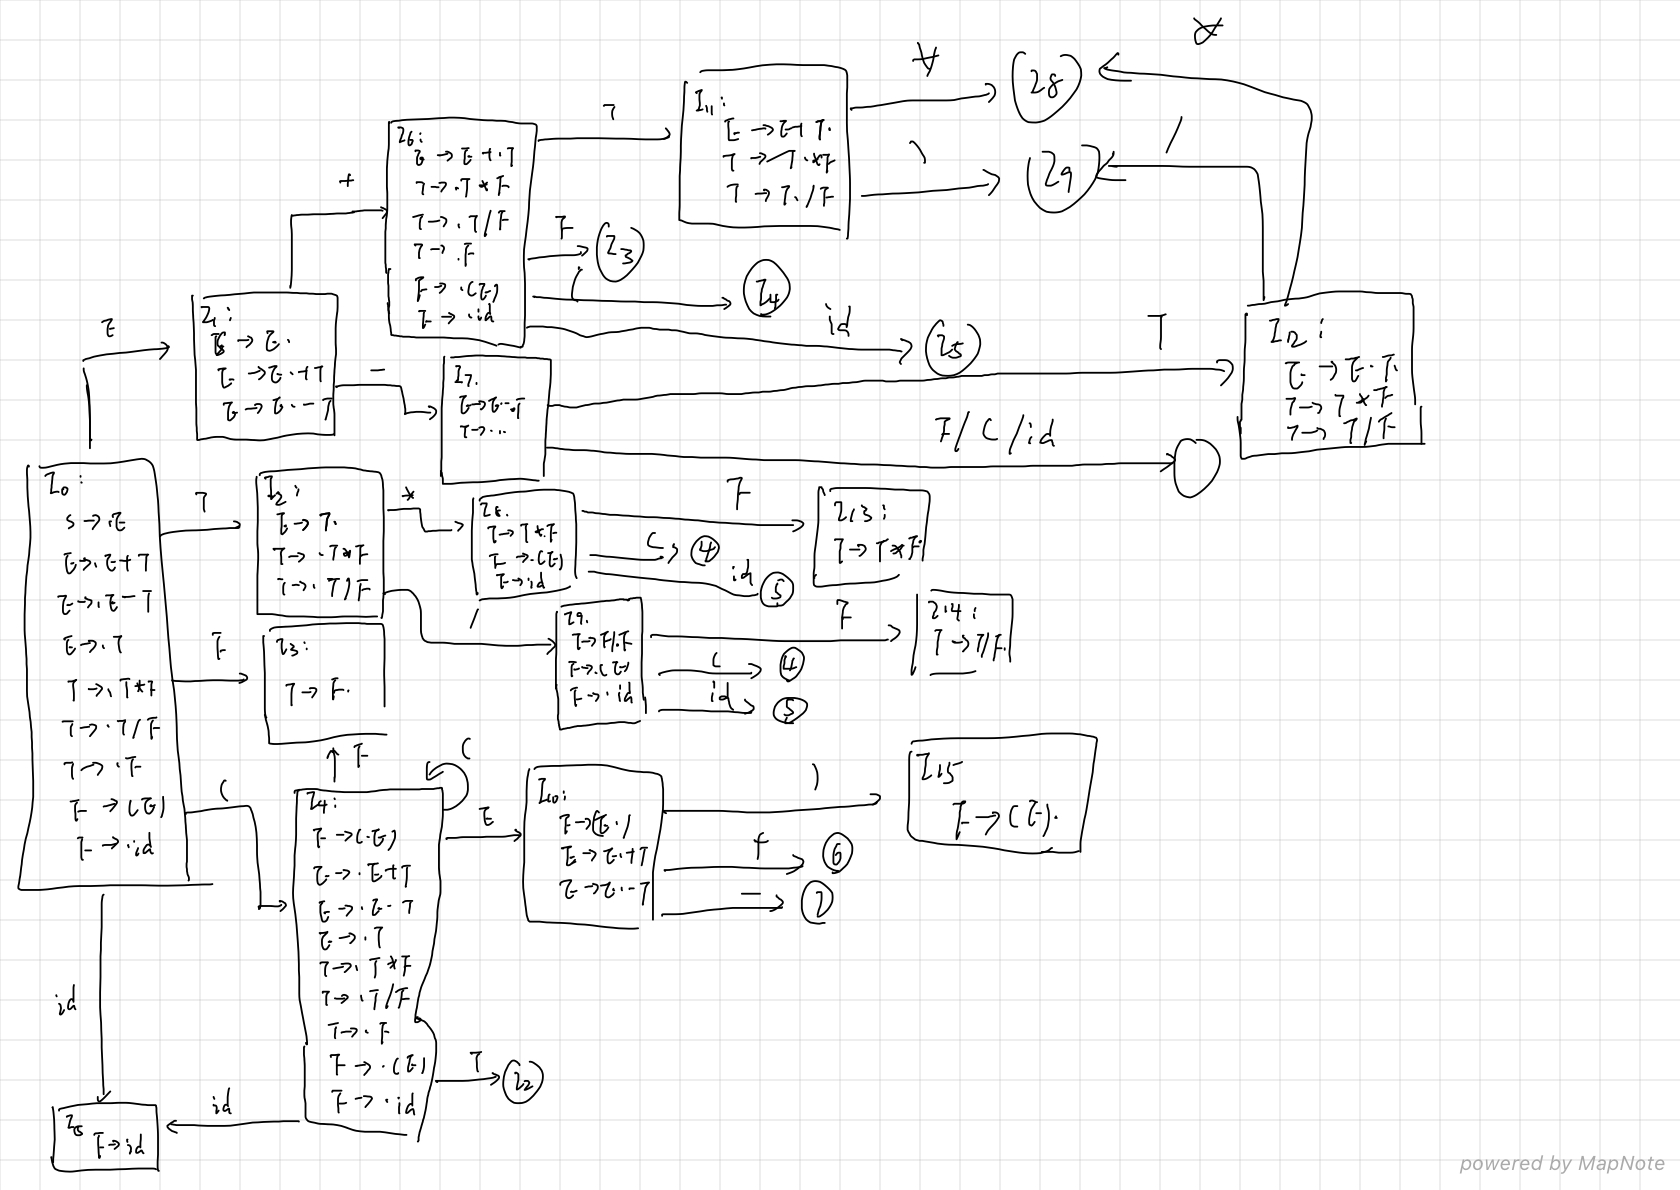
\includegraphics[width=.9\textwidth]{DFA.png}
    \caption{构造 DFA}
    \label{fig:5}
\end{figure}

可以发现,DFA 中存在移进-规约冲突,因此我们使用 $SLR(1)$
进行语法分析,构造的分析表如下一页表格所示。

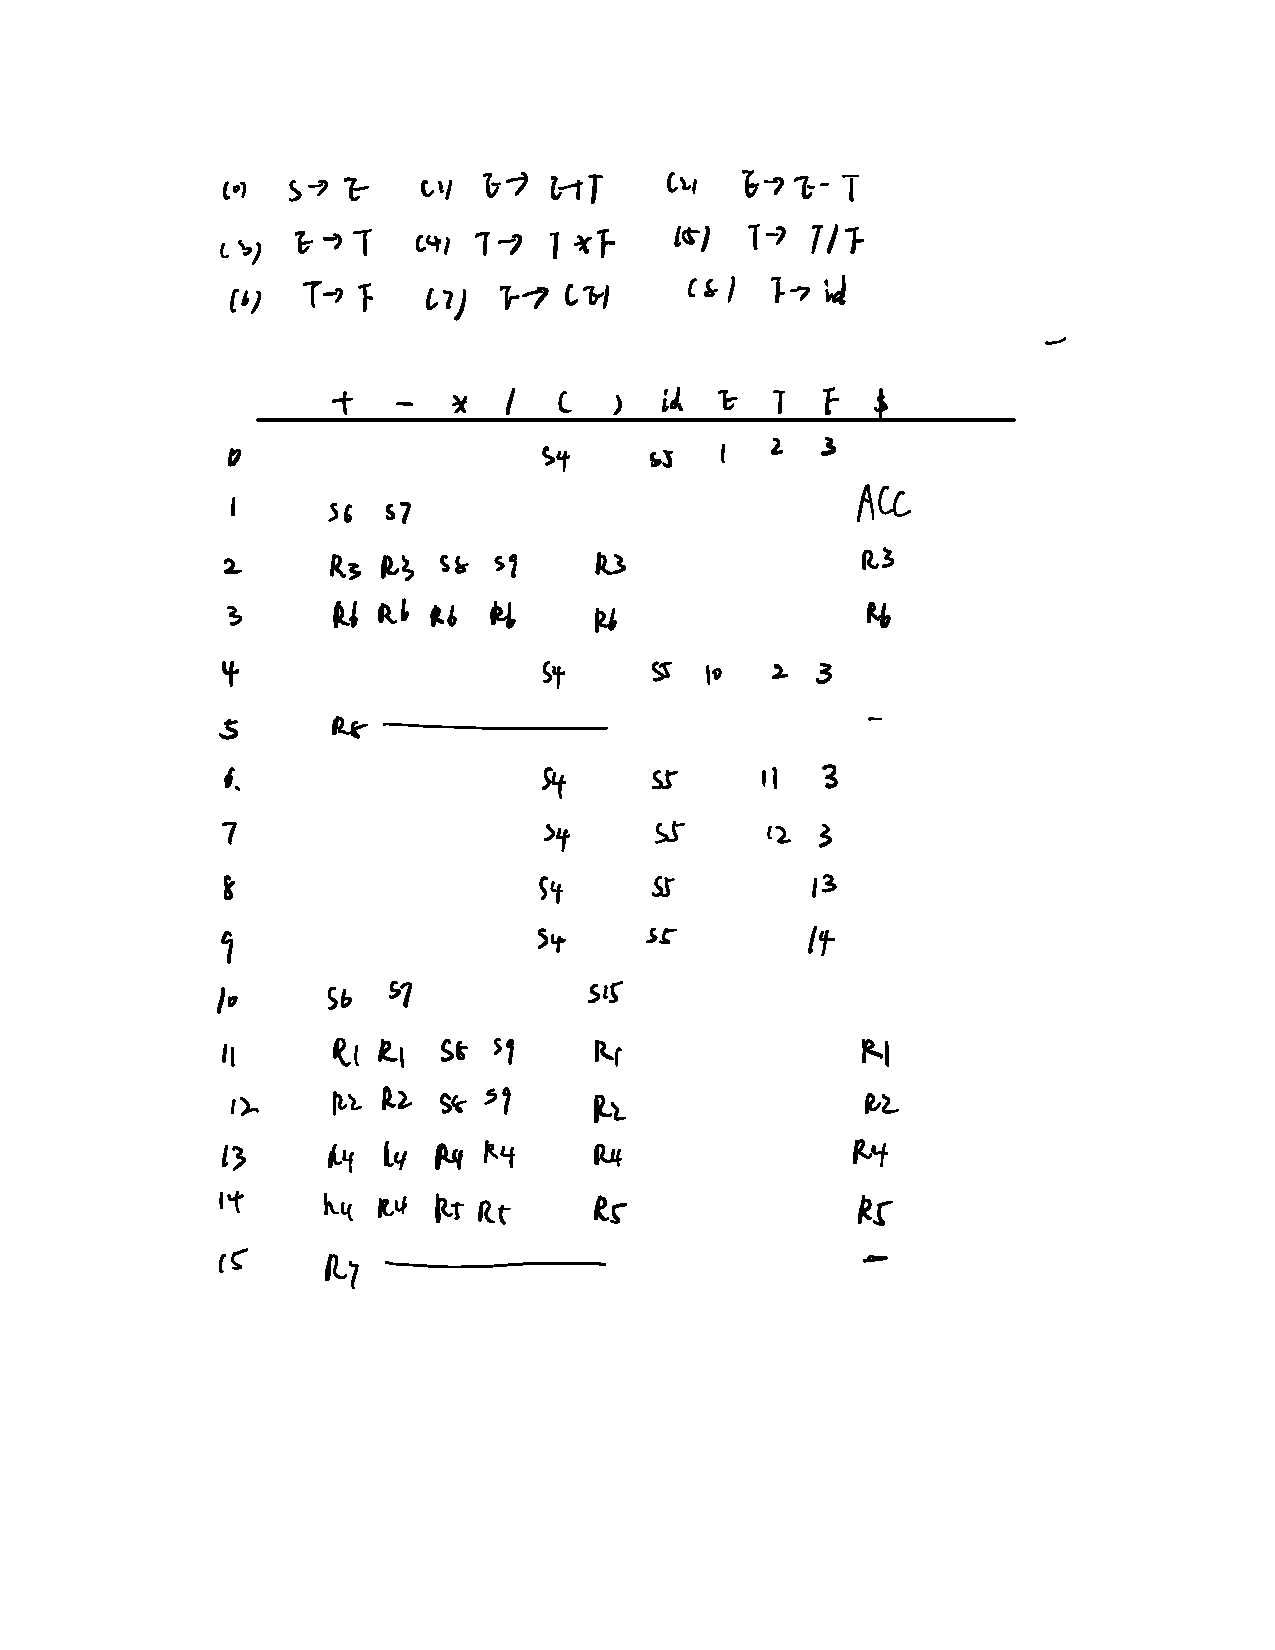
\includepdf[pages={1}]{LR1/986AEEC0-1B65-4601-A871-8B0EED40AF13.pdf}

\subsection{实验代码}
解析算法与书上一致。主要代码如下:
\lstinputlisting[language=python]{LR1/LR1.py}

\subsection{运行结果}

我们以解析 \texttt{(1 + 2) * 3 - 4} 为例,程序的输出如下:

\begin{lstlisting}
PS D:\playground\FuckingCalculator> python .\LR1\LR1.py
[(0, '')]
0, -- (
[(0, ''), (4, '(')]
4,( -- n
[(0, ''), (4, '('), (5, 'n')]
5,n -- +
F->n
[(0, ''), (4, '('), (3, 'F')]
3,F -- +
T->F
[(0, ''), (4, '('), (2, 'T')]
2,T -- +
E->T
[(0, ''), (4, '('), (10, 'E')]
10,E -- +
[(0, ''), (4, '('), (10, 'E'), (6, '+')]
6,+ -- n
[(0, ''), (4, '('), (10, 'E'), (6, '+'), (5, 'n')]
5,n -- )
F->n
[(0, ''), (4, '('), (10, 'E'), (6, '+'), (3, 'F')]
3,F -- )
T->F
[(0, ''), (4, '('), (10, 'E'), (6, '+'), (11, 'T')]
11,T -- )
E->E+T
[(0, ''), (4, '('), (10, 'E')]
10,E -- )
[(0, ''), (4, '('), (10, 'E'), (15, ')')]
15,) -- *
F->(E)
[(0, ''), (3, 'F')]
3,F -- *
T->F
[(0, ''), (2, 'T')]
2,T -- *
[(0, ''), (2, 'T'), (8, '*')]
8,* -- n
[(0, ''), (2, 'T'), (8, '*'), (5, 'n')]
5,n -- -
F->n
[(0, ''), (2, 'T'), (8, '*'), (13, 'F')]
13,F -- -
T->T*F
[(0, ''), (2, 'T')]
2,T -- -
E->T
[(0, ''), (1, 'E')]
1,E -- -
[(0, ''), (1, 'E'), (7, '-')]
7,- -- n
[(0, ''), (1, 'E'), (7, '-'), (5, 'n')]
5,n -- $
F->n
[(0, ''), (1, 'E'), (7, '-'), (3, 'F')]
3,F -- $
T->F
[(0, ''), (1, 'E'), (7, '-'), (12, 'T')]
12,T -- $
E->E-T
[(0, ''), (1, 'E')]
1,E -- $
S->E
\end{lstlisting}

\section{实验总结}
在这次实验中,我实现了$LL(1)$ 以及 $SLR(1)$ 进行
表达式的语法解析。通过这次实验,我对课本上的理论内容
有了更深刻的理解。

\end{document}